%%%%%%%%%%%%%%%%%%%%%%%%%%%%%%%%%%%%%%%%%%%%%%%%%%%%%%%%
% Este é um documento que servirá de modelo para
% os relatórios feitos na disciplina Laboratório de Circuitos Lógicos
% 2020-2
%%%%%%%%%%%%%%%%%%%%%%%%%%%%%%%%%%%%%%%%%%%%%%%%%%%%%%%%%

%%%%%%%%%%%%%%%%%%%%%%%%%%%%%%%%%%%%%%%%%%%%%%%%%%%%%%%%%
% Use os diferentes diretórios para colocar os relatórios de cada experimento, deste modo vc consegue manter um histórico e todo material organizado em apenas um local.
% Lembre-se de mudar o Main Document no Menu!!!

\documentclass[12pt]{article}

\usepackage{sbc-template}
\usepackage[brazil,american]{babel}
\usepackage[utf8]{inputenc}

\usepackage{graphicx}
\usepackage{url}
\usepackage{float}
\usepackage{listings}
\usepackage{color}
\usepackage{todonotes}
\usepackage{algorithmic}
\usepackage{algorithm}
\usepackage{hyperref}
\usepackage{amsmath}
\usepackage{graphicx}
\usepackage{array}
\usepackage[shortlabels]{enumitem}

\sloppy


\title{Experimento 4\\
Circuitos Combinacionais: Comparador de Palavras}

\author{Matheus Cardoso de Souza, 202033507\\
        Ualiton Ventura da Silva, 202033580\\
        Grupo G42
}

%%%% LEMBRE-SE DE MUDAR O GRUPO NA LINHA ABAIXO!!!!! %%%%%%
\address{Dep. Ciência da Computação -- Universidade de Brasília (UnB)\\
  CIC0231 - Laboratório de Circuitos Lógicos
  \email{matheus-cardoso.mc@aluno.unb.br, 202033580@aluno.unb.br}
}

\begin{document}
\maketitle

\selectlanguage{american}
 \begin{abstract}
   The current report aims to show off the elaboration of comparative circuits
   using concepts already presented in previous reports, like Karnaugh maps,
   boolean functions e their simplifications, as well as analyze the achieved
   results and delays due to mechanical factors inherent to the digital
   micro-architecture.
 \end{abstract}
\selectlanguage{brazil}

 \begin{resumo}
   O presente relatório tem como objetivo a elaboração de circuitos comparadores
   utilizando conceitos já apresentados como mapa de Karnaugh e funções
   booleanas e suas simplificações, assim como a análise de seus resultados e
   atrasos obtidos por fatores mecânicos existentes na microarquitetura digital.
 \end{resumo}


\section{Introdução}
\label{sec:Introducao}

% Escreva com suas palavras o que vai ser trabalhado no experimento. Aqui temos um exemplo de como citar a bibliografia consultada \cite{boulic:91} \cite{smith:99}.

Portas lógicas possuem a característica de poderem se combinar de diferentes
maneiras para a formulação de novos circuitos, a depender da maneira a qual se
combinam temos um circuito combinacional, que não retém memória de seus estados
anteriores. Contudo, ao ocorrer a associação destas portas lógicas, não será
obtido um sistema inafetado por erros, pois é necessária a consideração de
fatores mecânicos e como eles prejudicam a execução de um dado circuito, seja
ele combinacional ou não.

\subsection{Objetivos}
\label{sec:Objetivos}

O atual experimento busca não somente criar e demonstrar novos tipos de
combinações para a obtenção de comportamentos específicos e desejados, como
também fatores a serem considerados referentes ao tempo de resposta de um dado
sistema e porque ocorrem atrasos ao associar inumeras portas lógicas.

\subsection{Materiais}
\label{sec:Materiais}
Em função da natureza do ensino a distância, os presentes experimentos não foram
realizados usando-se materiais e equipamentos físicos, mas sim emulados por meio
do \href{https://www.digitalelectronicsdeeds.com/deeds.html}{Deeds}.

A seguir estão enumerados os materiais utilizados:
\begin{itemize}
    \item Componentes de Entrada(Gerador de clock e chave de estado)
    \item Componentes de Saída
    \item Portas Lógicas \textbf{NAND}, \textbf{OR}, \textbf{AND}, \textbf{NOT}
\end{itemize}

\section{Procedimentos}
\label{sec:Procedimentos}

Passaremos a apresentar os experimentos requeridos.

\subsection{Atraso de Propagação em portas lógicas}\label{sec:atraso_de_propagação}

\begin{enumerate}[A)]
\item \textbf{Equações Lógicas de L0 e L1}
\end{enumerate}

Começaremos com a equação lógica \textbf{L1}, pois \textbf{L0} depende dessa. Temos que, como
o número de portas \textbf{NOT} que ligam o sinal de clock \textbf{A} à
\textbf{L1} é \emph{ímpar}, a saída terá o sinal de \textbf{A} negado. Sendo
assim, concluímos que a equação para \textbf{L1} será:

\begin{equation}
L1 = \overline{A}
\end{equation}

Agora, considerando a saída \textbf{L0}, podemos verificar que existe uma porta
\textbf{AND} tomando o resultado de \textbf{A} e \textbf{L1}. Portanto, a equação de \textbf{L0} será:

\begin{equation}
L0 = A \cdot L1\label{eq:L0}
\end{equation}

Dessa forma, podemos expressar ambos \textbf{L0} e \textbf{L1} por meio de uma
tabela verdade, em função de \textbf{A}.

\begin{table}[H]
    \centering
    \caption{\textbf{L0} e \textbf{L1} em função de \textbf{A}}
    \begin{tabular}{|c|c|c|}\hline
        \multicolumn{1}{|c|}{Entrada} & \multicolumn{2}{|c|}{Saídas} \\\hline
        \textbf{A} & \textbf{L0} & \textbf{L1} \\\hline
        0 & 0 & 1 \\\hline
        1 & 0 & 0 \\\hline
    \end{tabular}\label{tab:atraso_de_propagação:L0_L1}
\end{table}

\begin{enumerate}[B)]
\item \textbf{Comportamento de L0 e L1}
\end{enumerate}

Utilizando a ferramenta
\href{https://www.digitalelectronicsdeeds.com/deeds.html}{Deeds} para a
simulação do circuito lógico, podemos observar que as saídas de \textbf{L0} e
\textbf{L1} são exatamente as esperadas quando leva-se em conta a tabela verdade
\ref{tab:atraso_de_propagação:L0_L1} apresentada acima.

Como representado nas figuras a seguir, o output de \textbf{L0} é \emph{sempre}
igual a $0$, e o output de \textbf{L1} é \emph{sempre} o oposto de \textbf{A},
assim como esperado.

\begin{figure}[H]
    \centering
    \includegraphics[width=.9\textwidth]{Exp04/exp4_2.0_b_clk_up_phone.png}
    \caption{Clock Up}\label{fig:exp4_2.0_b_clk_up_phone.png}
\end{figure}

\begin{figure}[H]
    \centering
    \includegraphics[width=.9\textwidth]{Exp04/exp4_2.0_b_clk_down_phone.png}
    \caption{Clock Down}\label{fig:exp4_2.0_b_clk_down_phone.png}
\end{figure}

\begin{enumerate}[C)]
\item \textbf{Formas de onda para L0 e L1}
\end{enumerate}

Utilizando a ferramenta \emph{Timing Diagram Simulation} podemos gerar as
formas de onda para \textbf{L0} e \textbf{L1}. A seguir reproduzimos as mesmas.

\begin{figure}[H]
    \centering
    \includegraphics[width=1\textwidth]{Exp04/exp4_2.0_c_clk_wave_phone.png}
    \caption{Onda e comprimento de pulso em \textbf{L0}}\label{fig:exp4_2.0_c_clk_wave_phone.png}
\end{figure}

Como pode-se observar, a saída \textbf{L0} possui um pequeno pulso quando o
clock varia. Podemos explicar esse comportamento levando em consideração o delay
que as portas lógicas possuem. Como a porta lógica \textbf{L0} possui como um de
seus inputs a porta \textbf{L1}, que por sua vez tem um delay de $5$ portas
\textbf{NOT}, a porta \textbf{L0} soma um delay de $5$ portas \textbf{NOT} e $1$
porta \textbf{AND}. Dessa forma, a soma total resulta em um delay de $21ns$,
como pode-se ver na imagem a seguir.

\begin{figure}[H]
    \centering
    \includegraphics[width=.9\textwidth]{Exp04/exp4_2.0_c_clk_wave_lenght_phone.png}
    \caption{Comprimento do pulso em \textbf{L0}}\label{fig:exp4_2.0_c_clk_wave_lenght_phone.png}
\end{figure}

\begin{enumerate}[D)]
\item \textbf{Pulsos em L0 quando A retorna ao nível 0}
\end{enumerate}

De forma sucinta, podemos afirmar que, para o circuito específico deste
exercício, contendo $5$ portas \textbf{NOT} e $1$ porta \textbf{AND}, não existe
pulso em \textbf{L0} quando \textbf{A} retorna ao nível $0$. O motivo para isso
é simples: quando \textbf{A} está retornando de $1$ para $0$ o valor lógico de
\textbf{L1} é $0$, e assim a porta lógica \textbf{AND} que produz o output de
\textbf{L0} sempre retornará o valor $0$, justificando a ausência de pulso nesse
momento do circuito.

Para justificar tal afirmação precisamos considerar qual a função lógica
responsável por produzir o output em \textbf{L0}. Lembrando da equação
\ref{eq:L0}, vemos que a única forma de termos um pulso em \textbf{L0} seria se
\textbf{L1} fosse $1$ no momento que \textbf{A} retorna ao nível $0$. Podemos
afirmar isso pois consideramos o delay da porta \textbf{AND} responsável pelo
output de \textbf{L0}. Logo, o pulso seria consideravelmente menor que o
existente na passagem de nível lógico \textbf{A} $= \, 0$ para \textbf{A}
$= \, 1$, mas seria possível existir. Cabe ressaltar, entretanto, que o pulso em
\textbf{L0} \emph{não} aconteceria na montagem de apenas $5$ portas
\textbf{NOT}, pois o delay não seria sufucientemente grande. Na imagem a seguir
apresentamos uma possível configuração de circuito lógico, contendo um número
\emph{ímpar} de portas \textbf{NOT}, que tem de fato um pulso em \textbf{L0}
quando \textbf{A} está retornando ao nível $0$.

\begin{figure}[H]
    \centering
    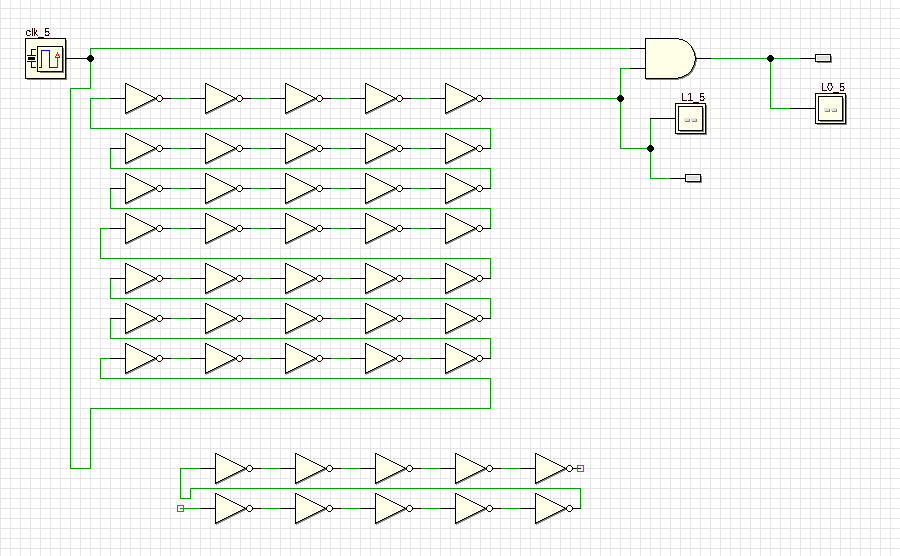
\includegraphics[width=.9\textwidth]{Exp04/exp4_2.0_d_clk_circuito_ao_voltar_para_zero.png}
    \caption{Circuito que apresenta pulso quando \textbf{A} retorna ao nível 0}\label{fig:exp4_2.0_d_clk_circuito_ao_voltar_para_zero.png}
\end{figure}

\begin{figure}[H]
    \centering
    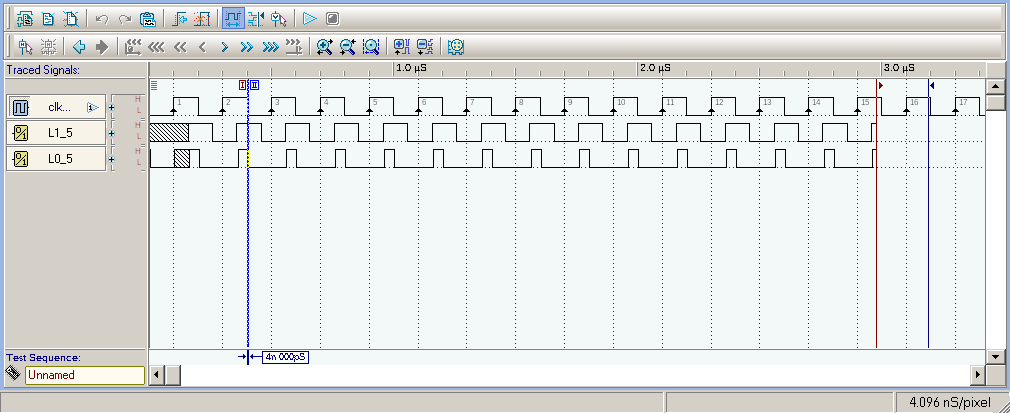
\includegraphics[width=.9\textwidth]{Exp04/exp4_2.0_d_clk_wave_ao_voltar_para_zero.png}
    \caption{Formato de onda desse circuito}\label{fig:exp4_2.0_d_clk_wave_ao_voltar_para_zero.png}
\end{figure}

\begin{figure}[H]
    \centering
    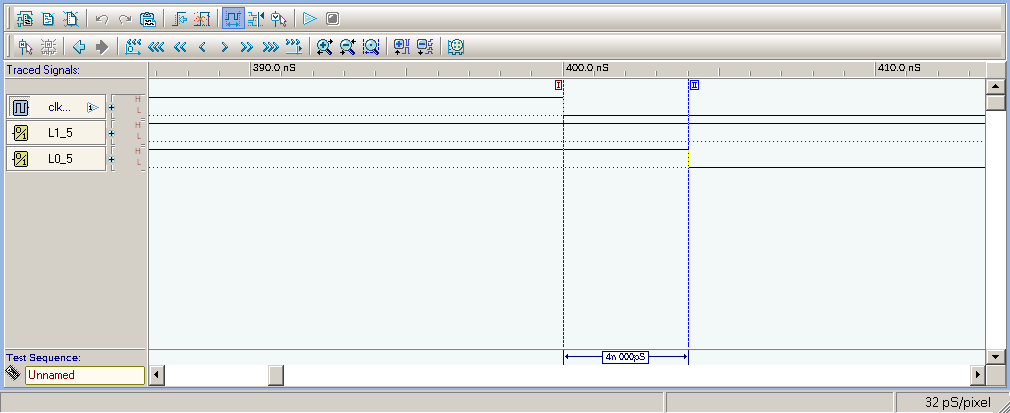
\includegraphics[width=.9\textwidth]{Exp04/exp4_2.0_d_clk_wave_lenght_ao_voltar_para_zero.png}
    \caption{Tamanho do pulso existente quando \textbf{A} retorna ao nível 0}\label{fig:exp4_2.0_d_clk_wave_lenght_ao_voltar_para_zero.png}
\end{figure}

\begin{enumerate}[E)]
\item \textbf{Haveria pulso em L0 caso houvesse um número par de portas NOT?}
\end{enumerate}

Sim, poderia existir um pulso em \textbf{L0}. O único limitante para a
observação de pulsos é a quantidade de portas \textbf{NOT} existentes no
circuito. O motivo é o mesmo do item anterior: quanto maior o número de portas,
maior será o delay no circuito lógico; Caso o delay acarrete em uma superposição
entre o nível lógico $1$ de \textbf{A} e \textbf{L1}, então haverá um pulso em
\textbf{L0}. Ou seja, o pulso é apenas limitado à introdução de um delay
suficientemente grande no circuito.

Como prova dessa afirmação, é apresentado um circuito com número \emph{par} de
portas \textbf{NOT}, e que ainda assim possui pulsos em \textbf{L0}.

\begin{figure}[H]
    \centering
    \includegraphics[width=.9\textwidth]{Exp04/exp4_2.0_e_clk_circuito.png}
    \caption{Circuito com pulso em \textbf{L0} usando número \emph{par} de portas \textbf{NOT}}\label{fig:exp4_2.0_e_clk_circuito.png}
\end{figure}

\begin{figure}[H]
    \centering
    \includegraphics[width=.9\textwidth]{Exp04/exp4_2.0_e_clk_circuito_wave.png}
    \caption{Formato de onda do circuito com pulso}\label{fig:exp4_2.0_e_clk_circuito_wave.png}
\end{figure}


\subsection{Comparador de palavras de \(3\) \emph{bits}}\label{sec:comparador_de_palavras_3_bits}

\begin{enumerate}[A)]
\item \textbf{Completando a tabela verdade para um circuito \textbf{XNOR}}
\end{enumerate}

Para fazermos a tabela verdade do circuito proposto no enunciado, basta notarmos
a própria definição de uma porta \textbf{XNOR}; Sendo assim, teremos:

\begin{table}[H]
    \centering
    \caption{Tabela Verdade para o circuito \textbf{XNOR}}
    \begin{tabular}{|c|c|c|c|c|}\hline
    \multicolumn{2}{|c|}{Entradas} & \multicolumn{1}{|c|}{Saída} \\\hline
    $A_{i}$ & $B_{i}$ & $Z_{i}$ \\\hline
    0 & 0 & 1 \\\hline
    0 & 1 & 0 \\\hline
    1 & 0 & 0 \\\hline
    1 & 1 & 1 \\\hline
    \end{tabular}\label{tab:comparador_de_palavras_3_bits}
\end{table}

\begin{enumerate}[B)]
\item \textbf{Implementação da função lógica $Z_{i}$ apenas com portas NAND}
\end{enumerate}

Para implementarmos um circuito lógico \textbf{XNOR} usando apenas portas
\textbf{NAND}, podemos usar o circuito a seguir:

\begin{equation}
\overline{\left( \overline{(\overline{A_{i} \cdot A_{i}}) \cdot (\overline{B_{i} \cdot B_{i}})} \right) \cdot (\overline{A_{i} \cdot B_{i}})}
\end{equation}

\begin{enumerate}[C)]
\item \textbf{TODO}
\end{enumerate}

  \textbf{TODO FALTA O LINK BOLADÃOOOOOOOOOOOOOOOOOOOOOOOOOOOOOOOOOOOO}

\begin{enumerate}[D)]
\item \textbf{Circuito comparador de palavras de 3 bits}
\end{enumerate}

Para montarmos o circuito total pedido no enunciado, basta usarmos $3$ dos
blocos implementados no item anterior, fazendo um \textbf{AND} entre cada uma
das $3$ saídas. Caso cada um dos blocos retorne o nível lógico $1$, então
teremos que o output final também será com nível lógico $1$, e, caso contrário,
o nível $0$. Existe, entretanto, um requisito: devemos montar esse circuito
apenas com portas \textbf{NAND} de $2$ entradas; Sendo assim, apresentamos um
circuito que satisfaz os requisitos necessários para o objetivo desejado:

\begin{figure}[H]
    \centering
    \includegraphics[width=.9\textwidth]{Exp04/exp4_2.1_d_circuito.png}
    \caption{Circuito Comparador de palavras de 3 bits}\label{fig:exp4_2.1_d_circuito.png}
\end{figure}

Reproduzimos a seguir a tabela verdade do circuito final. Contudo, Faz-se
necessário uma ressalva: como o circuito final possui $6$ valores de input, isso
acarreta em uma tabela com $2^{6} = 64$ linhas. Uma tabela assim seria muito
grande para reproduzirmos aqui. Dessa forma, optamos por somente mostrar os
inputs que produzem um output com valor igual a $1$. Todas as demais combinações
são assumidas como produzindo o output de nível lógico $0$.

\begin{table}[H]
    \centering
    \caption{Tabela Verdade para o circuito geral}
    \begin{tabular}{|c|c|c|c|c|c|c|}\hline
    \multicolumn{6}{|c|}{Entradas} & \multicolumn{1}{|c|}{Saída} \\\hline
    $A_{1}$ & $A_{2}$ & $A_{3}$ & $B_{1}$ & $B_{2}$ & $B_{3}$ & $Z_{i}$ \\\hline
    0 & 0 & 0 & 0 & 0 & 0 & 1 \\\hline
    0 & 0 & 1 & 0 & 0 & 1 & 1 \\\hline
    0 & 1 & 0 & 0 & 1 & 0 & 1 \\\hline
    0 & 1 & 1 & 0 & 1 & 1 & 1 \\\hline
    1 & 0 & 0 & 1 & 0 & 0 & 1 \\\hline
    1 & 0 & 1 & 1 & 0 & 1 & 1 \\\hline
    1 & 1 & 0 & 1 & 1 & 0 & 1 \\\hline
    1 & 1 & 1 & 1 & 1 & 1 & 1 \\\hline
    \end{tabular}\label{tab:comparador_de_palavras_3_bits}
\end{table}


\begin{enumerate}[E)]
\item \textbf{Circuito comparador de palavras de 3 bits}
\end{enumerate}

  \textbf{TODO FALTA A EXPLICAÇÃO BOLADA!!!!!!!!!!!!!!!!!!!!!!!!!!!!!!!!!!!!!!!!}

\subsection{Comparador de palavras de \(2\) \emph{bits}}\label{sec:comparador_de_palavras_3_bits}

\begin{enumerate}[A)]
\item \textbf{Tabela verdade de um comparador de 1 bit}
\end{enumerate}

Como trata-se de um comparador de 1 bit, para a tabela verdade teremos:

\begin{table}[H]
    \centering
    \caption{Tabela Verdade para o circuito comparador de 1 bit}
    \begin{tabular}{|c|c|c|c|c|}\hline
    \multicolumn{2}{|c|}{Entradas} & \multicolumn{3}{|c|}{Saída} \\\hline
    \textbf{$A$} & \textbf{$B$} & \textbf{$Y_{1}$} & \textbf{$Y_{2}$} & \textbf{$Y_{3}$} \\\hline
    0 & 0 & 0 & 1 & 0 \\\hline
    0 & 1 & 0 & 0 & 1\\\hline
    1 & 0 & 1 & 0 & 0\\\hline
    1 & 1 & 0 & 1 & 0\\\hline
    \end{tabular}\label{tab:comparador_de_palavras_3_bits}
\end{table}

Assim, terı́amos que para cada uma das saı́das desejadas, suas equações lógicas seriam:

\begin{equation}
Y_{1} = A \cdot \overline{B}
\end{equation}

\begin{equation}
Y_{2} = A \cdot B + \overline{A} \cdot \overline{B}
\end{equation}

\begin{equation}
Y_{3} = \overline{A} \cdot B
\end{equation}

Observa-se que todas as equações já estão em uma forma minimizada, já que possuem poucos termos, e quando colocadas em mapa de Karnaugh não haverá uma maneira de reduzi-las mais do que já descrito. Contudo, a minimização poderá ocorrer ao implementar o circuito.

\begin{enumerate}[B)]
\item \textbf{Implementação de um comparador de 1 bit}
\end{enumerate}

A principio, seguindo as equações de maneira literal teríamos o seguinte esquema:

\begin{figure}[H]
    \centering
    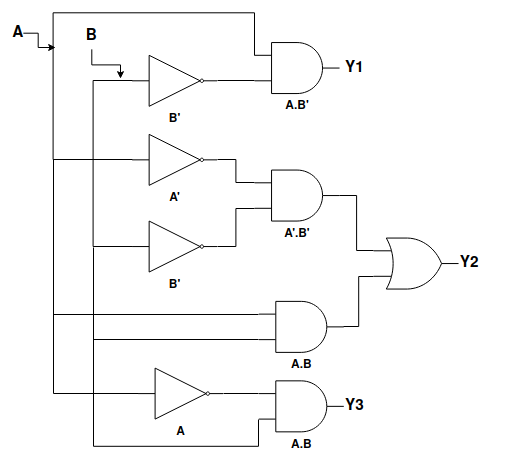
\includegraphics[width=.9\textwidth]{Exp04/Comparador1Bit.png}
    \caption{Comparador de 1 bit}\label{fig:Comparador1Bit.png}
\end{figure}

Uma maneira de criar redução será:
\begin{figure}[H]
    \centering
    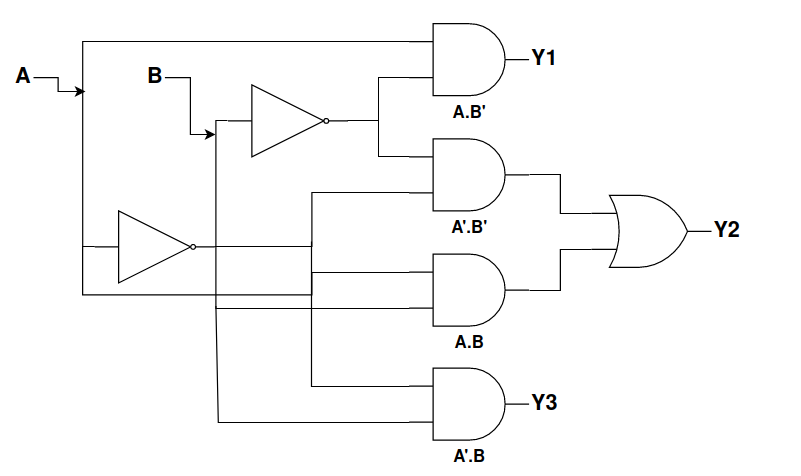
\includegraphics[width=.9\textwidth]{Exp04/Comparador1Simplificado.png}
    \caption{Comparador Simplificado de 1 bit}\label{fig:Comparador1Bit.png}
\end{figure}

Ou seja, bastando reduzir as portas \textbf{NOT} implementadas. Assim, temos que o subcircuito implementado através do Deeds será:

\begin{figure}[H]
    \centering
    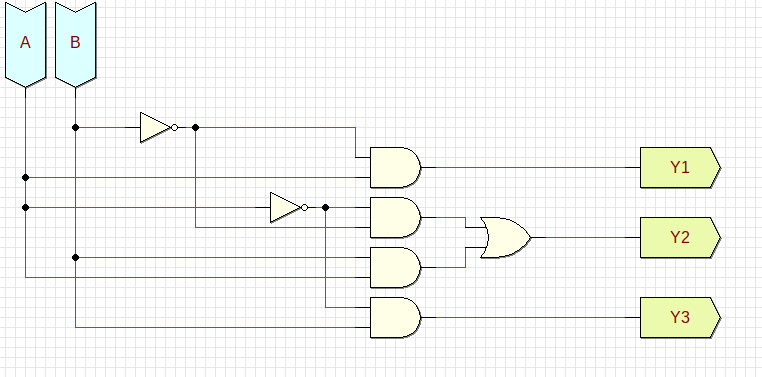
\includegraphics[width=.9\textwidth]{Exp04/Exp4.2.2.2.png}
    \caption{Comparador Simplificado de 1 bit - Deed}\label{fig:Comparador1Bit.png}
\end{figure}

Deve-se ater também ao fato de que por a utilização de duas portas \textbf{NOT} fatores como fan-out serão considerados.
Abaixo encontra-se o link de simulação:

"link bolado lindo perfeito QUERO CAFÉ"

\begin{enumerate}[C)]
\item \textbf{Implementação de um comparador de 2 bits}
\end{enumerate}

Utilizando o comparador de 1 bit construido, temos que a implementação para um comparador de 2 bits será:

IMAGEM

Abaixo segue o link de sua simulação:

"LINQUEEEEEEEEE EU QUERO CAFÉ"

Portanto, temos para sua tabela verdade o seguinte resultado:
\begin{table}[H]
    \centering
    \caption{Tabela Verdade para o circuito comparador de 2 bits}
    \begin{tabular}{|c|c|c|c|c|c|c|}\hline
    \multicolumn{4}{|c|}{Entradas} & \multicolumn{3}{|c|}{Saída} \\\hline
    \textbf{$A_{1}$} & \textbf{$A_{0}$} & \textbf{$B_{1}$} & \textbf{$B_{0}$} & \textbf{$Y_{1}$} & \textbf{$Y_{2}$} & \textbf{$Y_{3}$} \\\hline
    0 & 0 & 0 & 0 & 0 & 1 & 0\\\hline
    0 & 0 & 0 & 1 & 0 & 0 & 1\\\hline
    0 & 0 & 1 & 0 & 0 & 0 & 1\\\hline
    0 & 0 & 1 & 1 & 0 & 0 & 1\\\hline
    0 & 1 & 0 & 0 & 1 & 0 & 0\\\hline
    0 & 1 & 0 & 1 & 0 & 1 & 0\\\hline
    0 & 1 & 1 & 0 & 0 & 0 & 1\\\hline
    0 & 1 & 1 & 1 & 0 & 0 & 1\\\hline
    1 & 0 & 0 & 0 & 1 & 0 & 0\\\hline
    1 & 0 & 0 & 1 & 1 & 0 & 0\\\hline
    1 & 0 & 1 & 0 & 0 & 1 & 0\\\hline
    1 & 0 & 1 & 1 & 0 & 0 & 1\\\hline
    1 & 1 & 0 & 0 & 1 & 0 & 0\\\hline
    1 & 1 & 0 & 1 & 1 & 0 & 0\\\hline
    1 & 1 & 1 & 0 & 1 & 0 & 0\\\hline
    1 & 1 & 1 & 1 & 0 & 1 & 0\\\hline
    \end{tabular}\label{tab:comparador_de_palavras_3_bits}
\end{table}

\begin{enumerate}[D)]
\item \textbf{Atrasos Obtidos}
\end{enumerate}
Devido a estrutura de circuito feita, ocorrem longos atrasos, e que para o computadores utilizados contidianamente já seria um atraso significativo, percebe-se não somente problemas em seus atrasos como a produção de Hazards. Portanto, seria necessário uma análise mais detalhada que visa a redução destes erros.

\section{Análise dos Resultados}
\label{sec:Resultados}

Como pudemos notar através de todos os experimentos realizados erros e atrasos
ocorrem, provando a falha mecânica e a necessidade de técnicas que reduzam estes
mesmos erros. Percebe-se também como da transição de um estado booleano a outro
não irá produzir uma saída imediata, por fatores como o da própria borda de
subida e descida na mudança de estados. Importante notar que apesar do uso de um
simulador para os circuitos, ao utilizarmos geradores de onda no mundo físico,
deve-se considerar que não é possível a criação de estados de ondas que ocorrem
ao mesmo tempo, ou seja, simultâneos, pois, como já mencionado, sempre há
fatores mecânicos a serem considerados.

\section{Conclusão}
\label{sec:Conclusao}

A elaboração de técnicas que lidam com a álgebra booleana possibilitam
facilidade ao lidar com problemas do mundo real, de um ponto de vista teórico
foi possível a construção de modelos práticos. A principio poderia ser
percebidos como problemas futeis ou sem muitas necessidades, contudo, deve-se
notar que todos os computadores necessitam de tais operações, ou seja, igualdade
e inequações, assim, o presente relatório apesar de tratar destes problemas de
maneira mais simplificada ainda foi capaz de descrever comportamentos tão
desejados na implementação de máquinas utilizadas no dia a dia. Apesar de sermos
capazes de descrever tais comportamentos, deve-se notar que vêm com um preço,
sendo os erros associados a estes mesmos circuitos.

\nocite{*}
\bibliographystyle{sbc}
\bibliography{relatorio}  %Aqui é a definição do arquivo .bib a ser usado pelas referências


\newpage
% Colocar aqui apenas as respostas dos itens da Auto-Avaliação
\section*{Auto-Avaliação}

Respostas:
\begin{table}[H]
     \begin{tabular}{|c|c|} \hline
     \textbf{A} & \textbf{B}\\
     \hline
     1 & c \\ \hline
     2 & a \\ \hline
     3 & d \\ \hline
     4 & a \\ \hline
     5 & a \\ \hline
     \end{tabular}
\end{table}


\end{document}
